%%%%%%%%%%%%%%%%%%%%%%%%%%%%%%%%%%%%%%%%%%%%%%%%%%%%%%%%%%%%%%%%%%%%%%
% LaTeX Example: Project Report
%
% Source: http://www.howtotex.com
%
% Feel free to distribute this example, but please keep the referral
% to howtotex.com
% Date: March 2011 
% 
%%%%%%%%%%%%%%%%%%%%%%%%%%%%%%%%%%%%%%%%%%%%%%%%%%%%%%%%%%%%%%%%%%%%%%
% How to use writeLaTeX: 
%
% You edit the source code here on the left, and the preview on the
% right shows you the result within a few seconds.
%
% Bookmark this page and share the URL with your co-authors. They can
% edit at the same time!
%
% You can upload figures, bibliographies, custom classes and
% styles using the files menu.
%
% If you're new to LaTeX, the wikibook is a great place to start:
% http://en.wikibooks.org/wiki/LaTeX
%
%%%%%%%%%%%%%%%%%%%%%%%%%%%%%%%%%%%%%%%%%%%%%%%%%%%%%%%%%%%%%%%%%%%%%%
% Edit the title below to update the display in My Documents
%\title{Project Report}
%
%%% Preamble
\documentclass[paper=a4, fontsize=11pt]{scrartcl}
\usepackage[T1]{fontenc}
\usepackage{fourier}

\usepackage[english]{babel}															% English language/hyphenation
%\usepackage[protrusion=true,expansion=true]{microtype}	
\usepackage{amsmath,amsfonts,amsthm} % Math packages
\usepackage[pdftex]{graphicx}	
\usepackage{url}
\usepackage[utf8x]{inputenc} 
\setlength{\parindent}{0pt}
\setlength{\parskip}{0.5em}
\usepackage{pgfplots} 
\usepackage{listings}


%%% Custom sectioning
\usepackage{sectsty}
\allsectionsfont{\centering \normalfont\scshape}


%%% Custom headers/footers (fancyhdr package)
\usepackage{fancyhdr}
\pagestyle{fancyplain}
\fancyhead{}											% No page header
\fancyfoot[L]{}											% Empty 
\fancyfoot[C]{}											% Empty
\fancyfoot[R]{\thepage}									% Pagenumbering
\renewcommand{\headrulewidth}{0pt}			% Remove header underlines
\renewcommand{\footrulewidth}{0pt}				% Remove footer underlines
\setlength{\headheight}{13.6pt}


%%% Equation and float numbering
\numberwithin{equation}{section}		% Equationnumbering: section.eq#
\numberwithin{figure}{section}			% Figurenumbering: section.fig#
\numberwithin{table}{section}				% Tablenumbering: section.tab#


%%% Maketitle metadata
\newcommand{\horrule}[1]{\rule{\linewidth}{#1}} 	% Horizontal rule

\title{
		%\vspace{-1in} 	
		\usefont{OT1}{bch}{b}{n}
		\normalfont \normalsize \textsc{Università degli studi di Milano} \\ [25pt]
		\horrule{0.5pt} \\[0.4cm]
		\huge Algoritmi genetici con Mathematica: risoluzione del problema di Koza \\
		\horrule{2pt} \\[0.5cm]
}
\author{
		\normalfont 								\normalsize
        Claudio Chiappetta\\[-3pt]		\normalsize
        \today
}
\date{}


%%% Begin document
\begin{document}
\maketitle
\section{Il problema}
È stato scelto di risolvere un  noto problema nel campo dell'intelligenza artificiale, la cui prima formulazione si deve a John R. Koza.\cite{koza}


Si ha a disposizione un insieme di lettere, che opportunamente combinate formano una parola data. Nel nostro caso, seguendo la formulazione originaria di Koza, è stata scelta la parola "universal".

Queste lettere ("blocchi")sono suddivise in un insieme liberamente accessibile (il "tavolo"), e un insieme che si comporta come una pile (la "pila"). Si suppone inoltre di avere un "robot" che possa compiere determinate operazioni sui blocchi. Queste operazioni sono:
\begin{itemize}
\item {\textbf{ CS}} Ritorna l'elemento in cima alla pila.
\item {\textbf{ TB}} Ritorna l'ultimo elemento correttamente ordinato della pila.
\item {\textbf{ NN}} Ritorna la lettera successiva a \textbf{TB} nella parola "universal".
\item {\textbf{ MS}($x$)} Se $x$ è sul tavolo, sposta $x$ in cima alla pila e ritorna $x$.
\item {\textbf{ MT}($x$)} Se $x$ è nella pila, sposta sul tavolo l'ultimo elemento della pila, e ritorna $x$.
\item {\textbf{ DU}($esp1, esp2$)} Valuta $esp1$ finchè $esp2$ non diventa TRUE.
\item {\textbf{ NOT}($esp$)} Ritorna TRUE se $esp$ è uguale a NIL, altrimenti NIL.
\item {\textbf{ EQ}($esp1,esp2$)} Ritorna TRUE se le due espressioni sono uguali, NIL altrimenti
\end{itemize}

Tutte le funzioni ritornano NIL se incontrano problemi (ad esempio, se l'elemenot che dovrebbero ritornare non esiste).

Il problema consiste nello scrivere un algoritmo genetico che componga queste istruzioni per creare un programma che, se dato da eseguire al nostro robot, consenta al robot di scrivere la parola "universal" sullo stack, per qualsiasi configurazione iniziale delle lettere. In questo linguaggio, un programma corretto consiste in un set di comandi annidati (con una sola radice, che per convenzione viene scelta essere il comando EQ), dove ogni comando contiene il numero e il tipo corretto di argomenti. I primi tre comandi (detti "sensori") non accettano argomenti, i restanti prendono come argomento i singoli sensori oppure un set annidato di altri comandi, nel numero oportuno. 
Si nota che per forza di cose, i comandi "in fondo" al programma sono sensori.





\section{L'approccio}
Il problema è stato impostato in questo modo nel linguaggio di programmazione Mathematica. La pila e il tavolo sono stati rappresentati come variabili globali, nello specifico come liste contenenti le lettere della parola "universal".

I comandi del robot sono stati implementati come funzioni di Mathematica. 

Per quanto riguarda gli individui dell'algoritmo genetico, sono state percorse due strade.

La prima, la più semplice da implementare e sensibilmente più performante, sfrutta le potenzialità di Mathematica, ossia la possibilità di trattare ogni programma (un set di comandi annidati) come una lista annidata. Questo è vantaggioso perchè Mathematica mette a disposizione comandi ad alto livello per la manipolazione di liste ed alberi.

In questo modo un individuo non è altro che un espressione di Mathematica del tipo \texttt{C1[C2[], C3[..]]}, dove \texttt{C1,C2,C3...} sono le funzioni corrispondenti ai comandi del robot. È tuttavia necessario trovare un modo per bloccare la valutazione di questa espressione fino al momento opportuno, dal momento che Mathematica valuta le espressioni appena ne ha la possibilità.
  
Mathematica mette a disposizione dei comandi per controllare la valutazione delle espressioni, come ad esempio \texttt{Hold}, gli attributi \texttt{HoldAll} e simili, e altri comandi introdotti nelle versioni più recenti. È stato scelto di procedere in maniera meno ortodossa: ogni individuo è stato scritto utilizzando non le funzioni del robot definite in precedenza, ma funzioni "vuote" (non definite) con nomi simili; in questo modo l'espressione viene lasciata immutata (l'interprete non può valutare niente, perché le funzioni chiamate non sono definite), finché non viene usato il comando "ReplaceAll" per sostituire i nomi fittizi con le funzioni corrette, il che consente a Mathematica di procedere con la valutazione del programma

Si nota che i comandi specifici per il controllo della valutazione sono stati usati in altri punti del programma.

Come secondo approccio, per scopi puramente didattici, si è scelto di costruire e manipolare gli individui senza ricorrere alle potenzialità di Mathematica, ossia rinunciando alla possibilità di accedere ai livelli di una lista annidata e perfino senza conoscere a priori le dimensioni degli insiemi usati. Nonostante si sia cercato di costruire algoritmi efficienti, questi sono sensibilmente meno efficienti dei corrispondenti creati sfruttando Mathematica.

Un individuo di questo tipo è una lista con struttura ad albero, dove gli elementi al livello più basso (foglie) sono le funzioni che realizzano i sensori, ad esempio \texttt{Tb[] \&};  l'applicazione di una funzione ad una espressione si realizza mettendo nella prima posizione di una lista la funzione, e nelle restanti gli argomenti, ad esempio:  \texttt{EQ(CS NN) -> \{Eq[\#1,\#2] \&, Cs[] \&, Nn[] \& \} }.

A titolo di esempio, viene riportata la rappresentazione di  un insieme di istruzioni che svuotano la pila:

\[
\texttt{ \{DU[\#1, \#2] \& , \{MT[\#1] \& , CS[] \& \} , \{NOT[\#] \&,   \{NOT[\#] \&, CS[]\& \}\}\} }
\]

Questa struttura si presta maggiormente ad una generalizzazione, sia nel linguaggio (è più facilmente implementabile utilizzando linguaggi con meno funzionalità di Mathematica), sia nelle funzionalità, in quanto è possibile rappresentare un generico albero e affrontare così una ampia classe di problemi.

È stata creata una variabile globale per contenere il numero di passi effettuati dall'esecuzione di un individuo. In questo modo, oltre a misurare l'efficienza di un programma, è possibile bloccare l'esecuzione dei programmi che impieghino troppi passi, ed evitare loop infiniti, nonché garantire la creazione di una soluzione ragionevolmente efficiente.

Si è scelto di affidare l'incremento di questa variabile e il controllo sul numero di passi alle singole funzioni elementari. Questo perché, come viene mostrato nella sezione riguardante l'esecuzione degli individui, a causa dell'istruzione DU, è l'unico modo per escludere con certezza la possibilità di loop infiniti. 




\subsection{Generazione casuale degli individui iniziali}
In entrambi i casi, gli individui vengono generati tramite ricorsione. Prendiamo in considerazione il solo caso del secondo approccio (liste di funzioni). 

La funzione generatrice parte creando una lista di tre elementi, dove nella prima posizione viene messa la funzione \texttt{Eq[\#1,\#2] \&}, e nelle altre due viene chiamata una funzione che, in maniera random decide se ritornare un sensore, oppure ritornare una delle funzioni, e chiamare di nuovo se stessa per decidere l'argomento della funzione.

Inoltre, questa funzione generatrice controlla che vengano creati programmi corretti, ossia programmi in cui ogni comando ha argomenti del tipo corretto. L'unico comando con una restrizione sugli argomenti è il comando \texttt{DU}, che per evitare un sicuro loop infinito, richiede di avere come secondo argomento una proposizione (una sequenza di comandi che può ritornare \texttt{TRUE} o \texttt{NIL}. 

%possibile grafico

In questo modo, è possibile creare uniformemente programmi random, senza però vincoli sulla lunghezza. 
Se non si è interessati ad avere programmi particolarmente brevi, per controllarne la lunghezza è sufficiente scartare gli individui che superino un certo numero di nodi totale (il numero dato da \texttt{Length[Flatten[individuo]]}. 

In generale, generare programmi di lunghezza inferiore ad una soglia non è un problema banale, se si vuole che questo avvenga in un numero ragionevole di passi e senza \emph{bias} fra i rami.

Un metodo ingenuo potrebbe essere contare quanti nodi sono stati creati, e interrompere la generazione dopo una soglia. Questo metodo però non garantisce una distribuzione uniforme dei pezzi dell'albero.

È stato adottato un metodo basato sulla potatura (\emph{pruning}). Quando un programma supera la soglia di lunghezza, uno dei suoi rami (scelto casualmente) viene sostituito con una foglia casuale; il procedimento viene ripetuto finchè il programma non è sufficientemente corto. Questo è un algoritmo probabilistico, che non garantisce il raggiungimento dell'obbiettivo dopo un numero fissato di passi, ma che ha elevata probabilità di terminare in tempi brevi, e sicuramente non introduce bias fra le parti dell'albero.



\subsection{Esecuzione di un individuo}
Per gli individui del tipo 1, è sufficiente effettuare un \texttt{ReplaceAll}: \texttt{/.\{ nomefintoTB -> Tb, \dots  \}}

A questo punto il programma diventa un'espressione valutabile da Mathematica

Gli individui del tipo 2 vengono convertiti in individui del tipo 1 tramite una funzione ricorsiva \texttt{TreeToExp}, che funziona in questo modo: presa una lista che corrisponde all'esecuzione di una funzione \texttt{\{funzione , argomento1, argomento2   \}}, ritorna il primo elemento applicato all'esecuzione di \texttt{TreeToExp} agli elementi successivi: \texttt{funzione[TreeToExp[argomento1], TreeToExp[argomento2]}.
\texttt{TreeToExp} Applicata ad una foglia ritorna \texttt{nomefintosensore}

È interessante notare che, se non fosse per la presenza dell'istruzione \texttt{DU}, sarebbe immediato valutare un individuo di questo tipo senza dover passare per questa conversione; è sufficiente modificare la funzione \texttt{TreeToExp} in modo che valuti i sensori invece che sostituirli con espressioni da valutaere. In presenza di istruzioni che richiedono di valutare più di una volta le espressioni passate come argomento, non c'è un modo sempice per fare questo, neanche utilizzando le funzioni per il controllo della valutazione.

L'istruzione \texttt{DU} crea problemi anche nell'approccio 1; per garantire un'esecuzione corretta sono state necessarie alcune accortezze, fra cui l'uso dell'attributo \texttt{HoldAll} nella funzione \texttt{DU}.


\subsection{Fitness}
In maniera simile all'implementazione originaria di Koza, abbiamo scelto, per ogni esecuzione dell'algoritmo di generare un insieme di configurazione iniziali per le lettere (dell'ordine del centinaio di elementi), quasi tutte random tranne alcuni casi particolari fissati per tutte le esecuzioni.

Questi casi particolari sono gli stessi usati da Koza, ossia otto configurazioni in cui la pila contiene correttamente le prime $i$ lettere del bersaglio, con $i$ da $1$ a $8$, e altre otto in cui la situazione è quasi la stessa, ma la pila contiene anche una lettera casuale in testa. In più c'è una configurazione per cui il problema è già risolto.


Ogni programma viene eseguito per tutte le configurazioni iniziali, e la funzione di fitness ritorna il numero di configurazioni per cui il programma.

È stata implementata anche un'altra funzione di fitness che, dopo un esecuzione del programma con una delle configurazioni iniziali, assegnava un punto per ogni lettera ordinata nella pila, più un bonus se tutte le lettere venivano ordinate correttamente. Il punteggio totale è la somma di questo per tutte le configurazioni iniziali, come nel caso precedente.
 
Questa funzione è stata introdotta perchè, con un campione di configurazioni e/o individui limitato, sarebbe stato ragionevole supporre che la fitness originaria non fosse in grado di evidenziare differenze fra gli individui (generando un programma random, è improbabile che questo riesca ad ordinare una configurazione).

Tuttavia, l'utilizzo della fitness alternativa non ha migliorato il funzionamento del programa.

Infine, sempre sulla scia del lavoro di Koza, si è voluta scrivere una funzione di fitness che premiasse i programmi più efficienti. Questo è stato fatto in due modi:


Ricordiamo che Koza utilizza il termine \emph{efficiente} per indicare un programma che termina in pochi passi, e il termine "parsimonioso" per indicare un programma che utilizza pochi comandi.

In primo luogo è stata utilizzata la stessa fitness utilizzata storicamente da Koza, ossia una funzione che somma un punteggio da 0 a 70 basato sulla quantità di configurazioni correttamente ordinate dal programma (con lo stesso metodo usato dalla funzione "standard"),   e un punteggio da 0 a 15, dato con i seguenti criteri:
\begin{itemize}
\item Viene dato $0$ se il programma ha ottenuto meno di $75$ punti nella valutazione della correttezza.
\item Viene dato $0$ se il programma compie in media un numero di passi minore di $min_{passi}$ (il numero di passi usato in media dal programma più efficiente possibile) o maggiore di $max_{passi}$ (il massimo numero di passi considerato accettabile, a discrezione dello sviluppatore, in genere dell'ordine di $O(n^2)$, dove $n$ è la lunghezza della parola target.
\item Viene dato $25$ se il programma in media finisce in $min_{passi}$.
\item I punti vengono distribuiti linearmente fra i due estremi.
\end{itemize}

Inoltre, viene assegnato un punteggio da $0$ a $15$ per la parsimonia seguendo gli stessi criteri dell'efficienza, usando come numero minimo di comandi $12$, la lunghezza minima per una soluzione, e come numero massimo è stato scelto arbitrariamente $20$.

È anche stata implementata una variazione di questa funzione, che funziona in maniera quasi identica ma associa il punteggio per l'efficienza e la parsimonia anche a programmi che ordinano solo una parte delle configurazioni di test, proporzionatamente alla percentuale di configurazioni correttamente ordinate, in modo da evitare di premiare programmi brevi che non svolgono niente di utile.

\subsection{Crossover e mutazione}

Il metodo di Crossover usato, lo stesso in entrambi gli approcci, è lo stesso usato da Koza.

Una  mutazione  viene realizzata generando un albero casuale e sostituendolo ad un ramo dell'individuo scelto casualmente.

Per generare una coppia di figli a partire da due individui, si seleziona un ramo casuale dal primo individuo, e lo si sostituisce ad un ramo casuale del seconde; viceversa per il secondo figlio.

Tuttavia, l'implementazione di questo meccanismo è radicalmente diversa nei due approcci.

Nel primo approccio, ottenere  casualmente un ramo da un individuo è immediato; in Mathematica, l'ultimo livello di una lista contiene, nel nostro caso, tutti i rami dell'albero, presi una sola volta. È suficiente scegliere un elemento casuale di  questo insieme, che si ottiene con \texttt{Level[tree, -1]}.

Per inserire un dato ramo in un punto casuale dell'albero, si seleziona casualmente un ramo dell'albero originario, ne si trova la posizione con \texttt{Position}, e si usa il comando\texttt{ReplacePart} per inserire in quella posizione il nuovo ramo.

Nel caso del secondo approccio, la manipolazione degli alberi è meno immediata, dal momento che l'unica funzione che abbiamo a disposizione è la funzione \texttt{Part}, che consente di accedere agli elementi di una lista. Se si conosce il numero di nodi dell'albero, un modo per affrontare il problema potrebbe essere di decidere un modo di indicizzare l'albero, e trattare l'albero come una lista, costruendo opportune funzioni per accedere agli elementi con l'indicizzazione prescelta. 

Nel nostro caso è stato scelto un algoritmo del tipo \emph{Reservoir Sampling} che non richiede di conoscere la dimensione dell'albero, che garantisce in ogni caso un tempo di esecuzione $O(N)$.

Per selezionare un ramo casuale da un individuo, l'algoritmo percorre ricorsivamente tutti i nodi  dell'albero, mettendo il nodo corrente in una fissata variabile temporanea (il deposito) con probabilità $1/n$, dove $n$ è il numero corrente di passi. Alla fine viene restituita la variabile temporanea. Facendo i conti, si trova che ogni ramo dell'albero ha la stessa probabilità di essere scelto.

Si procede in maniera analoga per inserire un ramo in un punto casuale di un individuo dato, con la differenza che in questo caso bisogna avere qualche accortezza in più con la variabile di deposito, dal momento che tenere in memoria una posizione dell'albero (che non è indicizzato) non è un problema banale.

L'implementazione di questi due metodi rende evidenti i vantaggi di un linguaggio di manipolazione simbolica come Mathematica rispetto ad un linguaggio di basso livello. Il crossover realizzato con gli strumenti di Mathematica è più sintetico, più intuitivo e ha performances significativamente migliori.



\subsection{Riproduzione}

La prima generazione è composta da $n_{ind}$ individui generati casualmente, di lunghezza contenuta ($<25$ comandi). A partire da questa vengono scelti i genitori secondo il criterio \emph{fitness proportionate}, ossia viene creata una lista di $n_{ind} -2$, e viene riempita scegliendo elementi random della prima generazione, con probabilità proporzionale  alla loro fitness. 
Si sarebbero potuti prendere in considerazione anche altri criteri per la selezione dei genitori, ma dati i ragionevoli tempi di esecuzione dell'algoritmo, non è stato ritenuto necessario.

Questa lista di elementi (i "genitori") viene scorsa a coppie, e ogni coppia con una certa probabilità $p_c$  viene sostituita dalla coppia dei figli, ottenuti con il metodo descritto in precedenza. 

Questo processo genera $n_{ind}-2$ nuovi individui, per cui è necessatio agiungere altri due programmi. Questi vengono scelti essere i due individui con la fitness più alta nella generazione precedente.  Questa  modifica è molto importante per garantire una rapida convergenza dell'algoritmo. Esecuzioni del progamma senza questa caratteristica non convergevano in tempi ottimali ($\lesssim 100$ generazioni)

Successivamente a tutti gli individui viene applicata una mutazione, ossia con una propabilità pari a $p_m$ un ramo dell'individuo scelto casualmente viene sostituito con un ramo generato casualmente.



\section{Ottimizzazione dell'algoritmo e risultati}



Per prima cosa, è stato necessario determinare il valore dei parametri dell'algoritmo, $p_c$ e $p_m$.

Questi sono stati determinati empiricamente, eseguendo il programma con diverse combinazioni dei parametri in un intervallo ragionevole (sappiamo che nella maggior parte dei casi, un algoritmo genetico funziona in maniera ottimale quando $p_c  > 0.7$ e $p_m \sim 0.01$).

Il tempo di esecuzione del programma non è ovviamente deterministico, ma è soggetto a fluttuazioni statistiche. Non sono state eseguite sufficienti esecuzioni da permettere una statistica rigorosa su queste fluttuazioni e di conseguenza una stima precisa delle performance del programma. Considerati i tempi di esecuzione (dell'ordine di $1 \div 10$ ore per ogni esecuzione), una statistica rigorosa  avrebbe richiesto una quantità rilevante di tempo e risorse.

Dai dati raccolti, risulta che il programma converge più velocemente per bassi valori di $p_c$ ($p_c \sim 0.7$) e alti valori di $p_m$ ($p_m \sim 0.005$). Questo potrebbe significare che è il caso, più che l'evoluzione, a dettare la comparsa di soluzioni. 

Tuttavia, la convergenza  viene ottenuta dopo un numero di generazioni simile per tutti i parametri ($ \sim 20$ per le configurazioni ottimali, $\sim 30$ per quelle non ottimali). Inoltre in ogni singola esecuzione il massimo della fitness di ogni generazione è rigorosamente crescente, anche se non sempre convergente al massimo.


Per ogni valore dei parametri, l'algoritmo usualmente converge prima della quarantesima generazione. 

Rimane da discutere un aspetto del programma, ossia la generazione di programmi efficienti oltre che corretti.

Con una esecuzione ingenua dell'algoritmo, che non pone limiti stretti alla lunghezza iniziale dei programmi e non premia l'efficienza,  si nota un comportamento di questo tipo:
i valori della fitness rimangono molto bassi per gran parte della durata del programma, nelle ultime generazioni salgono rapidamente verso il massimo; vengono generati programmi molto lunghi che inevitabilmente generano loop infiniti. Si arriva ad una soluzione in un numero di generazioni ragionevole, ma le soluzioni trovate, sebbene svolgano il loro compito in un numero finito di passi, dopo avere ordinato le lettere proseguono in un loop presumibilmente infinito che non produce cambiamenti.

Se si prova a dare fitness nulla a tutti i programmi che eccedono il numero di passi $max_{passi}$ l'algoritmo non converge.

Per ottenere programmi migliori si è adottata la stessa strategia adottata da Joza, ossia:

\begin{itemize}
\item Limitare la lunghezza dei programmi iniziali, usando le tecniche discusse in precedenza.
\item Modificare la funzione \texttt{DU} del robot, in modo che si fermi dopo un numero fissato di iterazioni, scelto arbitrariamente in base alla lunghezza del bersaglio (è stato scelto $n=20$)
\item Scegliere una funzione di fitness che premiasse gli individui più efficienti (quelli che compiono un numero di passi vicino al minimo). Sono state usate le due funzioni descritte in precedenza.
\item Usare le stesse configurazioni iniziali usate da Koza, e la stessa dimensione della popolazione.
\item Lanciare l'algoritmo per un numero fissato di generazioni, invece che fermarlo quando genera il primo programma completo. È stato scelto di usare $200$ generazioni, che sembra essere sufficiente per stabilizzare la fitness (Koza ne usava $100$)
\end{itemize}

Utilizzando queste accortezze, l'algoritmo converge, portando a soluzioni che terminano in un numero finito di passi, ma solo se si utilizza la versione alternativa della fitness di Koza. Con la funzione di Koza, l'algoritmo produce solo soluzioni con punteggio di efficienza e parsimonia pari a $0$. 

Lanciando l'algoritmo con questa funzione di fitness, prima della generazione $50$ viene trovato un programma corretto, mentre prima della generazione $100$ la fitness degli individui si stabilizza intorno al suo valore massimo. Questo è in linea con i risultati ottenuti da Koza.

In figura \ref{fig::voti_pars} è rappresentato l'andamento del massimo valore della fitness in una singola esecuzione dell'algoritmo, notiamo che con questa configurazione ottimale l'andamento dei voti è simile a quello della configurazione ingenua. Il tempo di esecuzione medio è di circa $4$ ore.

Riportiamo uno degli individui generati con fitness massima ($96.63$)

\[
\texttt{EQ[DU[MT[CS[]], NOT[NOT[CS[]]]],
 DU[MS[NN[]], EQ[MS[NN[]], CS[]]]]}
\]
\begin{figure}
\label{fig::voti_pars}
\centering
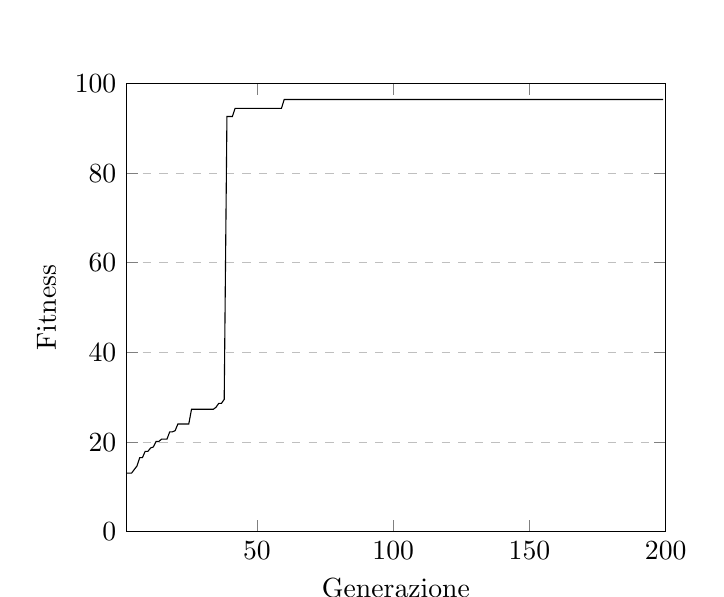
\begin{tikzpicture}
\begin{axis}[
    %title={Andamento del massimo voto assegnato in ogni generazione per generazion},
    xlabel={Generazione},
    ylabel={Fitness},
    xmin=2, xmax=200,
    ymin=0, ymax=100,
   % xtick={0,20,40,60,80,100},
   % ytick={0,20,40,60,80,100,120},
    legend pos=north west,
    ymajorgrids=true,
    grid style=dashed,
]
 
\addplot[
    %color=blue,
    %mark=*,
    ]
    coordinates { 
   (1., 11.94017094017094) (2., 13.070512820512821) (3., 13.070512820512821) 
 (4., 13.070512820512821) (5., 13.88034188034188) (6., 14.686507936507937) 
 (7., 16.542735042735043) (8., 16.542735042735043) 
 (9., 17.935897435897434) (10., 17.935897435897434) 
 (11., 18.694444444444443) (12., 18.923076923076923) 
 (13., 20.128205128205128) (14., 20.128205128205128) 
 (15., 20.666666666666668) (16., 20.666666666666668) 
 (17., 20.666666666666668) (18., 22.27905982905983) 
 (19., 22.27905982905983) (20., 22.566239316239315) 
 (21., 24.043162393162394) (22., 24.043162393162394) 
 (23., 24.043162393162394) (24., 24.043162393162394) 
 (25., 24.043162393162394) (26., 27.31893837156995) 
 (27., 27.31893837156995) (28., 27.31893837156995) 
 (29., 27.31893837156995) (30., 27.31893837156995) 
 (31., 27.31893837156995) (32., 27.31893837156995) 
 (33., 27.31893837156995) (34., 27.31893837156995) 
 (35., 27.779127305443094) (36., 28.65429599640126) 
 (37., 28.65429599640126) (38., 29.529464687359425) 
 (39., 92.61609686609687) (40., 92.61609686609687) 
 (41., 92.61609686609687) (42., 94.43660968660969) 
 (43., 94.43660968660969) (44., 94.43660968660969) 
 (45., 94.43660968660969) (46., 94.43660968660969) 
 (47., 94.43660968660969) (48., 94.43660968660969) 
 (49., 94.43660968660969) (50., 94.43660968660969) 
 (51., 94.43660968660969) (52., 94.43660968660969) 
 (53., 94.43660968660969) (54., 94.43660968660969) 
 (55., 94.43660968660969) (56., 94.43660968660969) 
 (57., 94.43660968660969) (58., 94.43660968660969) 
 (59., 94.43660968660969) (60., 96.41096866096866) 
 (61., 96.41096866096866) (62., 96.41096866096866) 
 (63., 96.41096866096866) (64., 96.41096866096866) 
 (65., 96.41096866096866) (66., 96.41096866096866) 
 (67., 96.41096866096866) (68., 96.41096866096866) 
 (69., 96.41096866096866) (70., 96.41096866096866) 
 (71., 96.41096866096866) (72., 96.41096866096866) 
 (73., 96.41096866096866) (74., 96.41096866096866) 
 (75., 96.41096866096866) (76., 96.41096866096866) 
 (77., 96.41096866096866) (78., 96.41096866096866) 
 (79., 96.41096866096866) (80., 96.41096866096866) 
 (81., 96.41096866096866) (82., 96.41096866096866) 
 (83., 96.41096866096866) (84., 96.41096866096866) 
 (85., 96.41096866096866) (86., 96.41096866096866) 
 (87., 96.41096866096866) (88., 96.41096866096866) 
 (89., 96.41096866096866) (90., 96.41096866096866) 
 (91., 96.41096866096866) (92., 96.41096866096866) 
 (93., 96.41096866096866) (94., 96.41096866096866) 
 (95., 96.41096866096866) (96., 96.41096866096866) 
 (97., 96.41096866096866) (98., 96.41096866096866) 
 (99., 96.41096866096866) (100., 96.41096866096866) 
 (101., 96.41096866096866) (102., 96.41096866096866) 
 (103., 96.41096866096866) (104., 96.41096866096866) 
 (105., 96.41096866096866) (106., 96.41096866096866) 
 (107., 96.41096866096866) (108., 96.41096866096866) 
 (109., 96.41096866096866) (110., 96.41096866096866) 
 (111., 96.41096866096866) (112., 96.41096866096866) 
 (113., 96.41096866096866) (114., 96.41096866096866) 
 (115., 96.41096866096866) (116., 96.41096866096866) 
 (117., 96.41096866096866) (118., 96.41096866096866) 
 (119., 96.41096866096866) (120., 96.41096866096866) 
 (121., 96.41096866096866) (122., 96.41096866096866) 
 (123., 96.41096866096866) (124., 96.41096866096866) 
 (125., 96.41096866096866) (126., 96.41096866096866) 
 (127., 96.41096866096866) (128., 96.41096866096866) 
 (129., 96.41096866096866) (130., 96.41096866096866) 
 (131., 96.41096866096866) (132., 96.41096866096866) 
 (133., 96.41096866096866) (134., 96.41096866096866) 
 (135., 96.41096866096866) (136., 96.41096866096866) 
 (137., 96.41096866096866) (138., 96.41096866096866) 
 (139., 96.41096866096866) (140., 96.41096866096866) 
 (141., 96.41096866096866) (142., 96.41096866096866) 
 (143., 96.41096866096866) (144., 96.41096866096866) 
 (145., 96.41096866096866) (146., 96.41096866096866) 
 (147., 96.41096866096866) (148., 96.41096866096866) 
 (149., 96.41096866096866) (150., 96.41096866096866) 
 (151., 96.41096866096866) (152., 96.41096866096866) 
 (153., 96.41096866096866) (154., 96.41096866096866) 
 (155., 96.41096866096866) (156., 96.41096866096866) 
 (157., 96.41096866096866) (158., 96.41096866096866) 
 (159., 96.41096866096866) (160., 96.41096866096866) 
 (161., 96.41096866096866) (162., 96.41096866096866) 
 (163., 96.41096866096866) (164., 96.41096866096866) 
 (165., 96.41096866096866) (166., 96.41096866096866) 
 (167., 96.41096866096866) (168., 96.41096866096866) 
 (169., 96.41096866096866) (170., 96.41096866096866) 
 (171., 96.41096866096866) (172., 96.41096866096866) 
 (173., 96.41096866096866) (174., 96.41096866096866) 
 (175., 96.41096866096866) (176., 96.41096866096866) 
 (177., 96.41096866096866) (178., 96.41096866096866) 
 (179., 96.41096866096866) (180., 96.41096866096866) 
 (181., 96.41096866096866) (182., 96.41096866096866) 
 (183., 96.41096866096866) (184., 96.41096866096866) 
 (185., 96.41096866096866) (186., 96.41096866096866) 
 (187., 96.41096866096866) (188., 96.41096866096866) 
 (189., 96.41096866096866) (190., 96.41096866096866) 
 (191., 96.41096866096866) (192., 96.41096866096866) 
 (193., 96.41096866096866) (194., 96.41096866096866) 
 (195., 96.41096866096866) (196., 96.41096866096866) 
 (197., 96.41096866096866) (198., 96.41096866096866) 
 (199., 96.41096866096866)
    
    };
    %\legend{CuSO$_4\cdot$5H$_2$O}
 
\end{axis}
\end{tikzpicture}

\caption{Andamento del massimo voto assegnato in ogni generazione per generazione, in una singola esecuzione dell'algoritmo, utlizzando una variazione della fitness di Koza}
\end{figure}


Cambiando la parola bersaglio diversa, l'algoritmo continua a convergere, se la parola bersaglio non contiene lettere ripetute. Anche Koza nella sua trattazione storica considera solo il caso di parole in cui ogni lettera compare una volta sola.
 
Il tempo e il numero di esecuzioni impiegati dall'algoritmo rimangono nello stesso ordine di grandezza a prescindere dalla lunghezza della parola bersaglio (intorno alle $4$ ore), anche se non sono state fatte abbastanza misurazioni per avere una statistica rigorosa. 




\section{Estensioni}
Come già anticipato, la struttura del programma è molto generale, e facilmente estensibile a diverse classi di problemi.

Lo stesso Joza ha usato questo tipo di algoritmo per risolvere una classe di problemi detti problemi di \emph{planning}, ossia problemi in cui si ha a disposizione un set di azioni che agiscono su di un sistema, e si vuole trovare una sequenza di azioni che raggiungano un certo obiettivo.

Una caratteristica che si può ricercare in un algoritmo che risolve problemi di planning è la robustezza delle soluzioni.

Per quanto riguarda il nostro algoritmo, abbiamo trovato che sia il programma che le soluzioni generate sono robuste; questo significa che le solizionitrovate per la parola "target" svolgono il loro compito con qualsiasi parola bersaglio, purchè la parola non contenga lettere ripetute, e l'algoritmo funziona correttamente anche se viene modificata la parola bersagio, sempre a patto che non contenga lettere ripetute.

Un'ulteriore generalizzazione non è immediatamente ottenibile, perchè i comandi del robottino non sarebbero adatti allo scopo.

Tuttavia, la struttura del programma è molto più generale di questo obiettivo, e con opportune modifiche ai comandi del robot permette di risolvere un generale problema di planning.

Inoltre, il tipo di struttura dati implementato nel secondo approccio consente di lavorare con qualsiasi dato si possa rappresentare con un albero, e quindi estendere l'applicazione dell'algoritmo genetico ad altri campi, come ad esempio l'interpretazione del linguaggio o l'allenamento di una rete neurale.




\begin{thebibliography}{55}
\bibitem{koza}  J. R. Koza, \emph{Genetic Programming: On the Programming of Computers by Means of Natural Selection} (MIT Press, Cambridge, MA, USA, 1992)

\bibitem{mitchell} M. Mitchell, \emph{An introduction to genetic algorithms} (MIT press, 1999)

\bibitem{spector} L. Spector, \emph{Genetic Programming and AI Planning Systems}, in \emph{Proceedings of the Twelfth National Conference on Artificial
Intelligence},  (AAAI Press/The MIT Press, 1994).

\bibitem{mcdermott} D. McDermott, \emph{The Current State Of Ai Planning Research}, in \emph{International Conference on Industrial and Engineering Applications of AI and Expert Systems}, 1994.


\end{thebibliography}

%%% End document
\end{document}